\begin{equation}
	\label{equ:equwave} 
	\derp{u}{x}{2} - \derp{u}{y}{2} = 0  \quad \mbox{или} \quad \derp{u}{t}{2} = a^2 \derp{u}{x}{2}
\end{equation}
	Простейшее уравнение гиперболического типа \eqref{equ:equwave} называют  \textit{уравнением колебаний струны}.\\
    
	Рассмотрим наиболее простую задачу о колебаних струны. Будем предполагать, что смещения струны лежат в одной плоскости и что вектор смещения $u$ перпендикулярен в любой момент времени к оси $x$; тогда процесс колебания можно описать одной функцией $u(x,t)$, характеризующей вертикальное перемещение струны. Будем рассматривать струну как гибкую упругую нить. Математическое выражение понятия гибкости заключается в том, что напряжения, возникающие в струне, всегда направлены по касательным к её мгновенному профилю (рис.\,\ref{fig:string}\!). Это условие выражает собой то, что струна не сопротивляется изгибу.
	\begin{figure}[h] 
		\centering 
		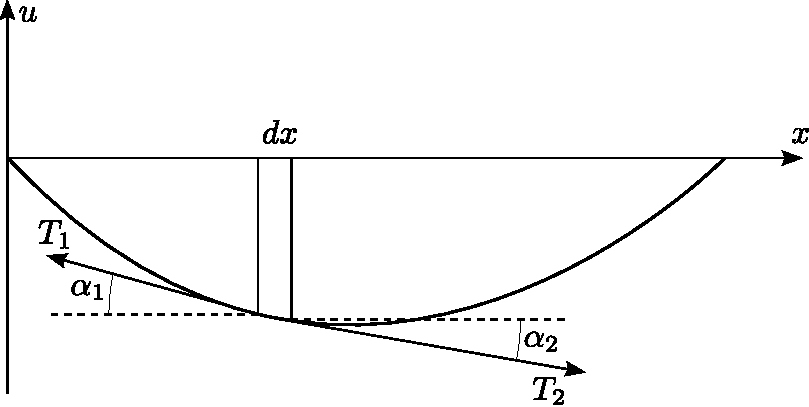
\includegraphics[scale=0.7]{string.pdf}  
		\caption{} \label{fig:string}
	\end{figure}

	Пусть $\rho$ -- линейная плотность струны, $a$ -- ускорение вдоль оси $x$:
	
	\[
		dm = \rho\, dx \quad a = \derp{x}{t}{2}
	\]
	Выделим бесконечно малый элемент струны и запишем II закон Ньютона:
	\[
		\rho \derp{x}{t}{2} dx = T_2 \cos \alpha_2 - T_1 \cos \alpha_1 = 0
	\]

	Пусть $\alpha_2, \alpha_1 \ll 1$, тогда $ \cos \alpha = 1 + O(\alpha^2). \quad T_2 = T_1 = T$\\
	Так как $\sum F_u \neq 0$, то 
	\[
		T_2 \sin \alpha_2 - T_1 \sin \alpha_1 = T (\alpha_2 - \alpha_1)
	\]
	Переходим к 
	\[
		\sin\alpha = \frac{\tg \alpha}{\sqrt{1 + \tg^2 \alpha}} = \frac{\derp{u}{x}{}}{\sqrt{1 + \left(\derp{u}{x}{}\right)^2}} \approx \derp{u}{x}{}
	\]
	\[
		\rho \derp{u}{t}{2} dx = T (\sin \alpha_2 - \sin \alpha_1) \approx  T \left( \derp{u}{x}{}\Bigl|_2 -  \derp{u}{x}{} \Bigl|_1 \right)
	\]
	Получаем уравнение  вида: 
	\[\rho \derp{u}{t}{2} = T \derp{u}{x}{2}\]
	В случае постоянной плотности $\rho = const$ это уравнение записывается в таком виде:\\
	\[\derp{u}{t}{2} = a^2 \derp{u}{x}{2}, \quad a = \sqrt{\frac{T}{\rho}}\]
